\textbf{Loading dataset}

I loaded 500 images of real faces and 500 images of spoof faces from the dataset.

\textbf{Raw pixel values}

The raw pixel values of the face images are used as features. I trained a Support Vector Machine (SVM) classifier on these raw pixel features to classify fake and real faces. The performance of the model on the dataset is portrayed in the code.

\textbf{Local Binary Patterns (LBP) features}

Local Binary Patterns (LBP) features are extracted from the face images for feature extraction. I trained an SVM classifier using the LBP features to classify fake and real faces. The performance of the model on the dataset is portrayed in the code.

\begin{figure}[H]
    \centering
    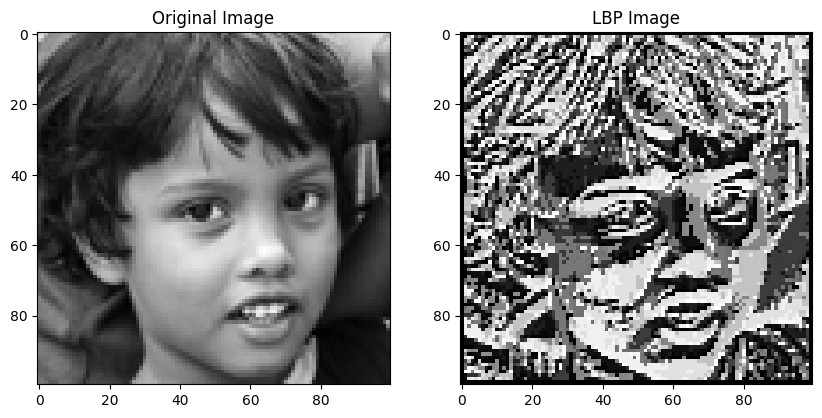
\includegraphics[width=.9\textwidth]{imgs/lbp.png}
    \caption{Local binary pattern}
    \label{fig:2_mediapipe}
\end{figure}

\newpage

\textbf{Edge methods}

Edge images are computed using the Prewitt and Sobel edge detectors. These edge images are used as input features independently to train an SVM classifier and classify fake and real faces. The performance of the model on the dataset is portrayed in the code.

\begin{figure}[H]
    \centering
    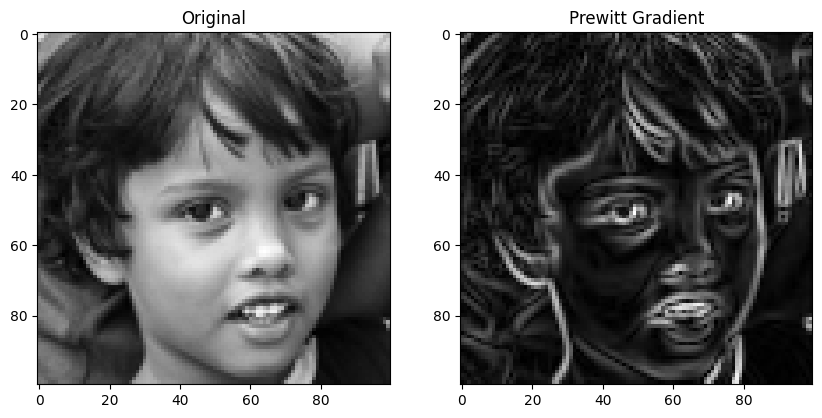
\includegraphics[width=.9\textwidth]{imgs/prewitt.png}
    \caption{Prewitt filtered image}
    \label{fig:2_mediapipe}
\end{figure}


\begin{figure}[H]
    \centering
    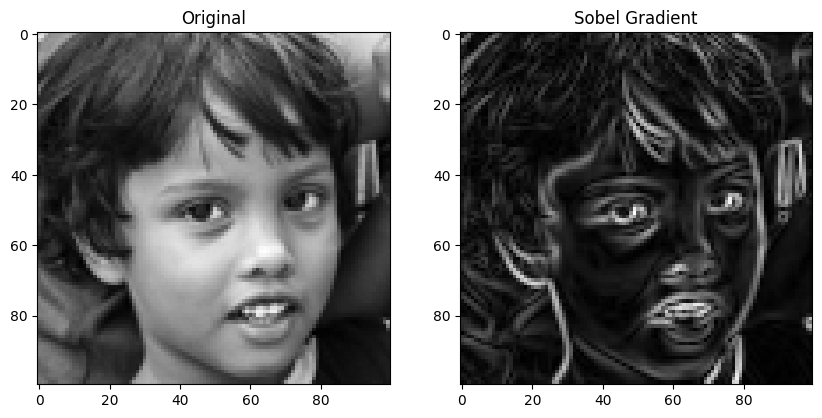
\includegraphics[width=.9\textwidth]{imgs/sobel.png}
    \caption{Sobel filtered image}
    \label{fig:2_mediapipe}
\end{figure}